\documentclass[a4paper]{article}

\usepackage{fullpage} % Package to use full page
\usepackage{parskip} % Package to tweak paragraph skipping
\usepackage{tikz} % Package for drawing
\usepackage{amsmath}
\usepackage{hyperref}
\usepackage{verbatimbox}
\usepackage{listings}
\usepackage{xcolor}
\usepackage{subfigure}

\definecolor{mygreen}{rgb}{0,0.6,0}
\definecolor{mygray}{rgb}{0.5,0.5,0.5}
\definecolor{mymauve}{rgb}{0.58,0,0.82}
\lstset{ %
  backgroundcolor=\color{white},   % choose the background color
  basicstyle=\footnotesize,        % size of fonts used for the code
  numberstyle=\tiny,
  breaklines=true,                 % automatic line breaking only at whitespace
  captionpos=b,                    % sets the caption-position to bottom
  commentstyle=\color{mygreen},    % comment style
  escapeinside={\%*}{*)},          % if you want to add LaTeX within your code
  keywordstyle=\color{blue},       % keyword style
  stringstyle=\color{mymauve},     % string literal style
}

\title{CSCE 569: Homework 3}
\author{Nick Tyler}
\date{03/30/18}

\begin{document}

\maketitle

\section*{Jacobi Iterative Method}


\begin{lstlisting}[language=C++]
while ((k <= mits) && (error > tol)) {
  error = 0.0;
#pragma omp parallel
  {
/* Copy new solution into old */
#pragma omp for private(i, j)
   for (i = 0; i < n; i++)
     for (j = 0; j < m; j++)
       uold[i][j] = u[i][j];
#pragma omp for private(i, j) reduction(+ : error)
   for (i = 1; i < (n - 1); i++) {
     for (j = 1; j < (m - 1); j++) {
       resid = (ax * (uold[i - 1][j] + uold[i + 1][j]) +
               ay * (uold[i][j - 1] + uold[i][j + 1]) + b * uold[i][j] -
               f[i][j]) / b;

       u[i][j] = uold[i][j] - omega * resid;
       error = error + resid * resid;
      }
   }
#pragma omp single nowait
   {
     if (k % 500 == 0)
       printf("Finished %ld iteration with error: %g\n", k, error);

     error = sqrt(error) / (n * m);
     k = k + 1;
    }
  } // End omp parallel region
}
\end{lstlisting}

\pagebreak
\begin{figure}[h]
%\subfigure[Execution time]{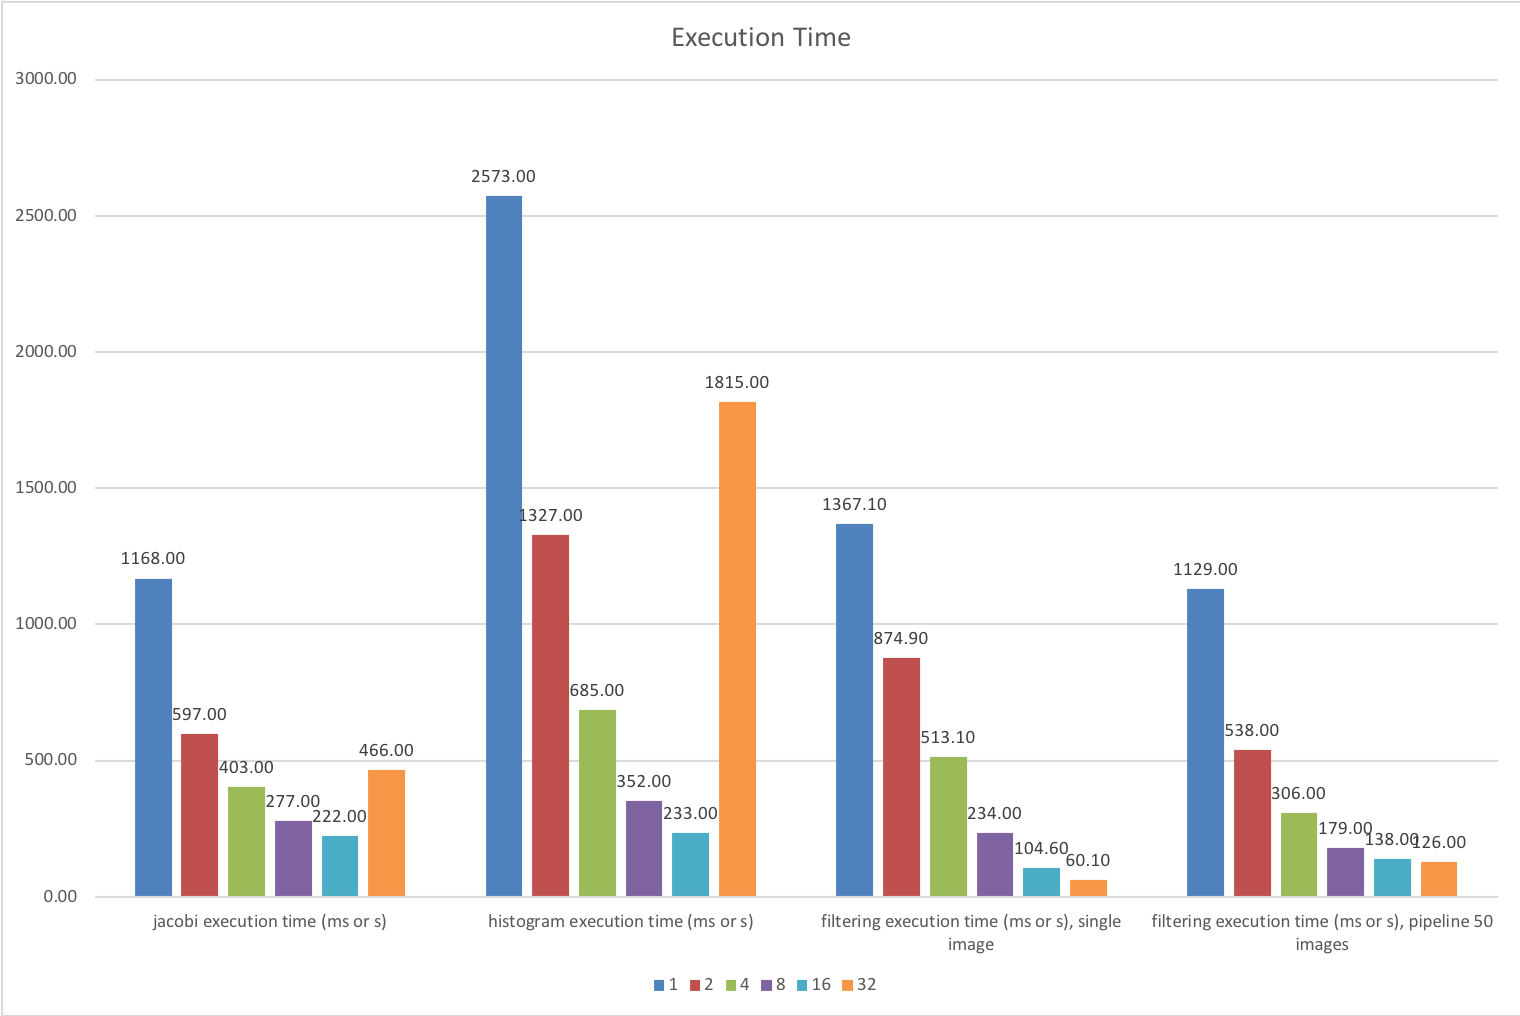
\includegraphics[scale=0.3]{bars.png}}
\vfill
%\subfigure[Speedup]{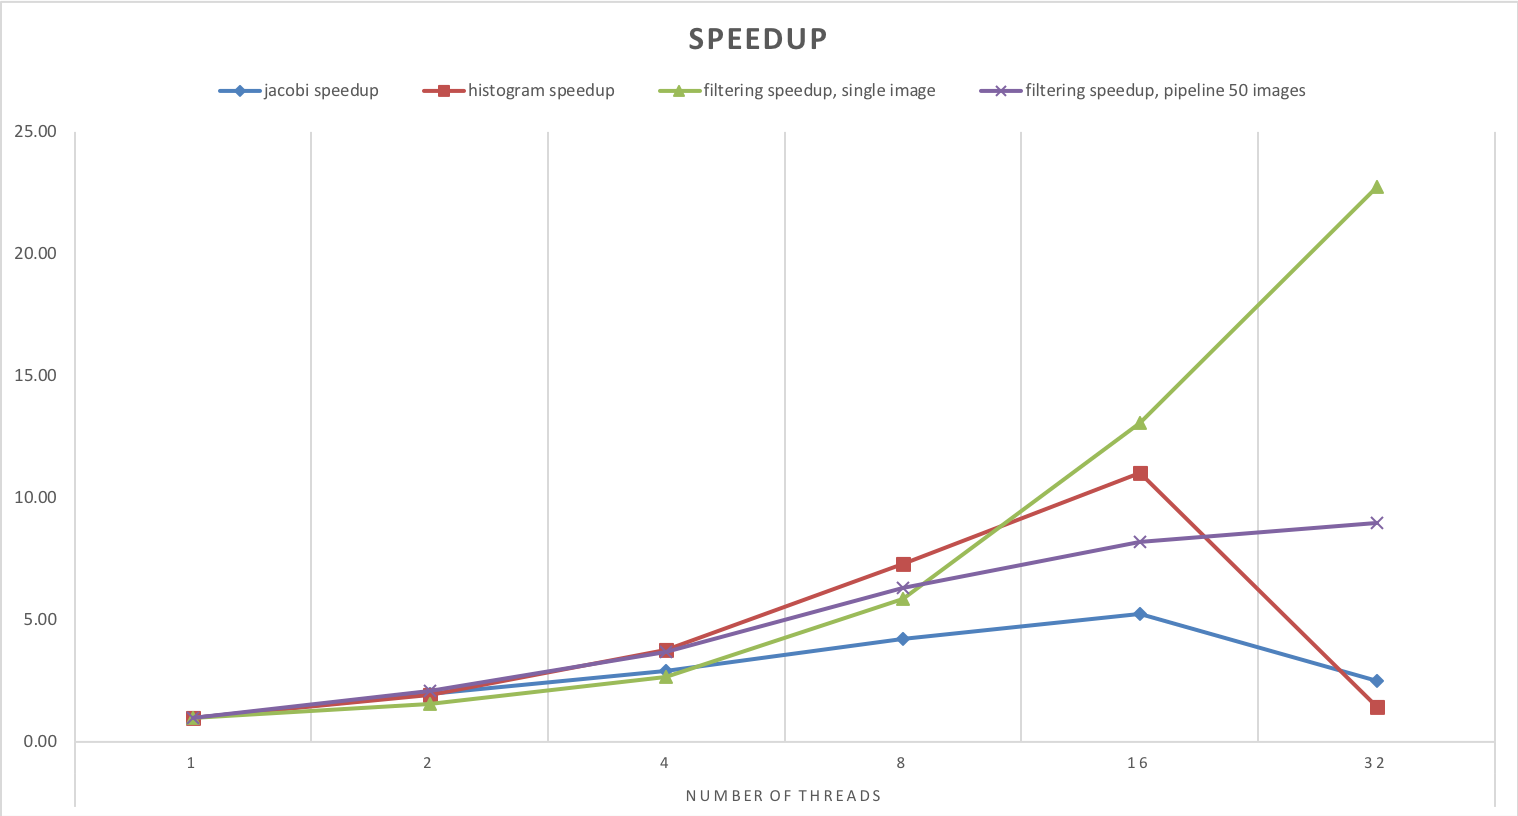
\includegraphics[scale=0.3]{lines.png}}
\caption{Performance Graphs}
\end{figure}


\end{document}
              
            
